% 	Name		:: 	sthlm Beamer Theme  HEAVILY based on the hsrmbeamer theme (Benjamin Weiss)
%	Author		:: 	Mark Hendry Olson (mark@hendryolson.com)
%	Created		::	2013-07-31
%	Updated		::	June 18, 2015 at 08:45
%	Version		:: 	1.0.2
%	Email		:: 	hendryolson@gmail.com
%	Website		:: 	http://v42.com
%
% 	License		:: 	This file may be distributed and/or modified under the
%                  	GNU Public License.
%
%	Description	::	This presentation is a demonstration of the sthlm beamer
%					theme, which is HEAVILY based on the HSRM beamer theme created by Benjamin Weiss
%					(benjamin.weiss@student.hs-rm.de), which can be found on GitHub
%					<https://github.com/hsrmbeamertheme/hsrmbeamertheme>.


%-=-=-=-=-=-=-=-=-=-=-=-=-=-=-=-=-=-=-=-=-=-=-=-=
%
%        LOADING DOCUMENT
%
%-=-=-=-=-=-=-=-=-=-=-=-=-=-=-=-=-=-=-=-=-=-=-=-=

\documentclass[newPxFont]{beamer}
\usetheme{sthlm}
%\usecolortheme{sthlmv42}

%-=-=-=-=-=-=-=-=-=-=-=-=-=-=-=-=-=-=-=-=-=-=-=-=
%        LOADING PACKAGES
%-=-=-=-=-=-=-=-=-=-=-=-=-=-=-=-=-=-=-=-=-=-=-=-=
\usepackage[utf8]{inputenc}
\usepackage[T1]{fontenc}

%\usepackage{chronology}
\usepackage{chronosys}
\usepackage{subfigure}

\newcommand{\tabitem}{%
  \usebeamertemplate{itemize item}\hspace*{\labelsep}}

%\renewcommand{\event}[3][e]{%
%  \pgfmathsetlength\xstop{(#2-\theyearstart)*\unit}%
%  \ifx #1e%
%    \draw[fill=black,draw=none,opacity=0.5]%
%      (\xstop, 0) circle (.2\unit)%
%      node[opacity=1,rotate=45,right=.2\unit] {#3};%
%  \else%
%    \pgfmathsetlength\xstart{(#1-\theyearstart)*\unit}%
%    \draw[fill=black,draw=none,opacity=0.5,rounded corners=.1\unit]%
%      (\xstart,-.1\unit) rectangle%
%      node[opacity=1,rotate=45,right=.2\unit] {#3} (\xstop,.1\unit);%
%  \fi}%

%-=-=-=-=-=-=-=-=-=-=-=-=-=-=-=-=-=-=-=-=-=-=-=-=
%        BEAMER OPTIONS
%-=-=-=-=-=-=-=-=-=-=-=-=-=-=-=-=-=-=-=-=-=-=-=-=

%\setbeameroption{show notes}

%-=-=-=-=-=-=-=-=-=-=-=-=-=-=-=-=-=-=-=-=-=-=-=-=
%
%	PRESENTATION INFORMATION
%
%-=-=-=-=-=-=-=-=-=-=-=-=-=-=-=-=-=-=-=-=-=-=-=-=

\title{Une approche par les Communs}
\subtitle{Ma vision}
%\date{\small{\jobname}}
%\date{\today}
\author{\texttt{E. Delay}, avec la participation de J.-P. Müller,\\
 une réflexion animée par \texttt{S. Aubert} et \texttt{A. Botta}}
\institute{CIRAD -- UMR SENS}

\hypersetup{
pdfauthor = {E. DELAY},
pdfsubject = {GRET Convention Programme 1},
pdfkeywords = {Atelier finale de la CP1)},
pdfmoddate= {D:\pdfdate},
pdfcreator = {}
}

\begin{document}

%-=-=-=-=-=-=-=-=-=-=-=-=-=-=-=-=-=-=-=-=-=-=-=-=
%
%	TITLE PAGE
%
%-=-=-=-=-=-=-=-=-=-=-=-=-=-=-=-=-=-=-=-=-=-=-=-=


\maketitle

%\begin{frame}[plain]
%	\titlepage
%\end{frame}

%-=-=-=-=-=-=-=-=-=-=-=-=-=-=-=-=-=-=-=-=-=-=-=-=
%
%	TABLE OF CONTENTS: OVERVIEW
%
%-=-=-=-=-=-=-=-=-=-=-=-=-=-=-=-=-=-=-=-=-=-=-=-=
% \section*{Une boussole ?}
% \begin{frame}{Overview}
% % For longer presentations use hideallsubsections option
% \tableofcontents[hideallsubsections]
% \end{frame}

%-=-=-=-=-=-=-=-=-=-=-=-=-=-=-=-=-=-=-=-=-=-=-=-=
%	FRAME: INTRODUCTION
%-=-=-=-=-=-=-=-=-=-=-=-=-=-=-=-=-=-=-=-=-=-=-=-=

\begin{frame}[c]{Une réflexion d'équipe}
\vspace{-1cm}
\begin{alertblock}{\textsc{ Sortie le 12 mai 2022}}
    Une actualité brulante de l'équipe !
\end{alertblock}
\begin{figure}
  \includegraphics[height=5cm]{img/communs_green_auteur.pdf}
\end{figure}
\end{frame}

\section{Introduction : modeliser dans l'urgence}


\begin{frame}[c]{L'urgence socio-environnementale}
\vspace{-1cm}
À l'échelle mondiale, de nombreux facteurs peuvent empêcher les populations d'avoir accès aux ressources fondamentales de leur existence :
\begin{itemize}
  \item faits de violence et de guerre,
  \item appropriation des terres au Sud,
  \item artificialisation au Nord,
  \item \textit{etc.}
\end{itemize}
\begin{figure}
  \includegraphics[height=3cm]{img/Honduras.jpg}
  \caption{\textit{Dépaysage au Honduras}, Agnès Stienne, 2019}
\end{figure}
\end{frame}

\begin{frame}[c]{Doomed ?}
\vspace{-1cm}

\begin{figure}
  \includegraphics[width=\textwidth]{img/im_legend-600.jpg}
  \caption{I'm a legend (film, 2007)}
\end{figure}
\end{frame}

\begin{frame}[c]{Un sentier, une piste, une autoroute ... ?}
\vspace{-1cm}
\begin{figure}
  \includegraphics[height=3.5cm]{img/cyrano.jpg}
  \caption{Cyrano de Bergerac (film 1990)}
\end{figure}
\begin{itemize}
  \item Depuis Ostrom (1990), une forte dynamique autour des Communs,
  \item Une dynamique qui réinterroge la condition de l’homme dans le système.
\end{itemize}
\end{frame}

\begin{frame}[c]{Mais pourquoi modéliser ?}
\vspace{-1cm}

Qu'est-ce qu'un modèle ?
\begin{itemize}
  \item `` A* est un modèle de A si manipuler A* permet de répondre à la question (ou l'objectif) Q sur A posée par X '' (Minsky 1965)
\end{itemize}

Pourquoi faire ?
\vspace{-0.4cm}
\begin{figure}
  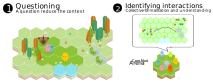
\includegraphics[height=3.2cm]{img/modeliser.png}
\end{figure}

\small{
  \begin{alertblock}{\textsc{Une hypothese forte}}
    La déconstruction de la réalité sous la forme abstraite de modèle va permettre aux différents acteurs concernés de mieux saisir et expliciter les relations entre les composants du système.
  \end{alertblock}
}
% \begin{figure}
%   \includegraphics[height=3.5cm]{img/pict_cyril_piou.jpg}~\includegraphics[height=3.5cm]{img/pict_etienne_delay.jpg}
% \end{figure}
\end{frame}

%-=-=-=-=-=-=-=-=-=-=-=-=-=-=-=-=-=-=-=-=-=-=-=-=
%	FRAME: LA NOTION DE SYSTÈME ET DE SYSTÈMES COMPLEXES
%-=-=-=-=-=-=-=-=-=-=-=-=-=-=-=-=-=-=-=-=-=-=-=-=

\section{L'apport des systèmes complexes}

\begin{frame}[c]{Le système et ses limites}
\vspace{-1cm}
Un système = (au moins) un observateur qui délimite
\begin{itemize}
  \item Posture réaliste : le système pré-existe à l'observateur et s'impose (Pseudo-communs (Theesfled, 2019))
  \item Posture épistémique : c'est l'observateur, la situation d'action, qui va délimiter le système (relation, interactions) (Ostrom, 1990; Haller, 2019).
\end{itemize}

\small{
  \begin{alertblock}{\textsc{Positionnement épistemique}}
      Le commun n'est pas, il devient.
  \end{alertblock}
}

En explicitant le système; son dedans et son dehors $\rightarrow$  conscientisation les limites est une condition nécessaire à sa définition.


\end{frame}

\begin{frame}[c]{Le système et les interactions}
\vspace{-1cm}
Un système c'est :
\begin{itemize}
  \item des composantes (humain et non humain)
  \item des relations entre ses composantes
\end{itemize}

\small{
  \begin{alertblock}{\textsc{Le système complexe}}
      \begin{itemize}
        \item Entrer par les relations structure des triptyques usagés $\rightarrow$ usage $\rightarrow$ ressource. La frontière se reconfigure au gré des interactions.
        \item Les interactions non linéaires ont la propriété de faire émerger un comportement au niveau du système considéré.
      \end{itemize}

  \end{alertblock}
}
\begin{figure}
  \includegraphics[height=3.5cm]{img/ReHab_network.png}
\end{figure}

\end{frame}


\begin{frame}[c]{Deux types d'emergence}
\vspace{-1cm}
On peut distinguer l’émergence faible de l’émergence forte

\begin{figure}
  \includegraphics[height=3.5cm]{img/Screenshot_2019-11-18 (143) Lucy's Famous Chocolate Scene - YouTube}
  \caption{Lucy's Famous Chocolate Scene (1950)}
\end{figure}

\small{
  \begin{alertblock}{\textsc{Auto-organisation}}
      L'émergence forte permet de maintenir les caractéristiques globales du système et donc les composants, leurs interactions et la frontière à l’origine de cette émergence.
  \end{alertblock}
}

\end{frame}

%-=-=-=-=-=-=-=-=-=-=-=-=-=-=-=-=-=-=-=-=-=-=-=-=
%	FRAME: GOUVERNER LES SYSTÈMES COMPLEXES
%-=-=-=-=-=-=-=-=-=-=-=-=-=-=-=-=-=-=-=-=-=-=-=-=

\section{Le GRET et la maturité des communs}

\begin{frame}[c]{La maturité des communs}
\vspace{-1cm}

Le GRET conçoit trois catégories de communs différents :
\begin{itemize}
    \item la ressource en tant que commun (nommé aussi “commun de ressource”),
    \item le service en tant que commun (ou “commun de service”)
    \item le territoire en tant que commun.
\end{itemize}

 \small{
   \begin{alertblock}{\textsc{Vers le territoire et au-delà}}
     On entre toujours par une ressource, autour de laquelle les utilisateurs se structurent pour petit à petit structurer un service (une émergence) et, quand plusieurs réseaux de communs se croisent sur un même territoire, on commence à identifier ce territoire comme un commun.
   \end{alertblock}
 }
\end{frame}

\begin{frame}[c]{L'acteur du vivre ensemble}
\vspace{-1cm}

\begin{itemize}
    \item Réaffirmer l’importance de la relation permet d’introduire un nouveau rôle dans le système : “l’acteur du vivre ensemble” (Aubert et Botta 2022), que Morizot (2020) décrit comme un “diplomate des relations”.
    \item Ce nouveau rôle ne cherche pas à préserver une entité du système, mais les relations qui unissent ces entités.
\end{itemize}

 \small{
   \begin{alertblock}{\textsc{Perturber le système}}
     Ce \textbf{changement de point de vue} implique un changement radical dans notre capacité d’observation du commun. C’est parce que nous sommes vigilants au maintien des relations que nous pouvons avoir une \textbf{analyse réflexive sur l’évolution et la maturité du commun}.
   \end{alertblock}
 }
\end{frame}

\begin{frame}[c]{Le GRET acteur du vivre ensemble}
\vspace{-1cm}

\begin{itemize}
    \item En se positionnant comme garant du maintien de cette relation, le GRET se situe d’un point de vue “politique” (au sens de H. Arendt 1958 (re-éd. 2020) ou de C. Mouffe, 2018)
    \item Cette progression vers un territoire en tant que commun va de pair avec une mise à jour dans l’espace public de ces réseaux de solidarité.
\end{itemize}
\begin{figure}
    \includegraphics[height=3.5cm]{img/atelier_montroland.jpg}
\end{figure}
\end{frame}


\begin{frame}[c]{Des formes de gouvernance : GIREL}
\vspace{-1cm}
\begin{itemize}
    \item Une entrée par la ressource eau, et des acteurs homogènes, puis une recherche de pluralité.
    \item plusieurs usages peuvent être concurrents : l’usage des maraîchers n’est par exemple pas le même que celui des éleveurs $\rightarrow$ service en temps que commun $\rightarrow$ De nouveaux attributs (suivi-évaluation)
\end{itemize}
\begin{figure}
    \includegraphics[height=3.5cm]{img/ComMod_f'eauDiem.png}
\end{figure}

\end{frame}

\begin{frame}[c]{Des formes de gouvernance : GPSE}
\vspace{-1cm}
\begin{itemize}
    \item La prise en compte de la pluralité des acteurs permet la coexistence de l’égalité (entre eux) et de la distinction (considérer chacun comme unique).
    \item Un \textbf{acteur du vivre ensemble} qui cherche a maintenir la relation entre usager et ressources, quelque soit le système autour (qualité de service)
\end{itemize}
 \small{
   \begin{alertblock}{\textsc{Qu'est-ce qui propulse le système : les valeurs }}
    Ces valeurs deviennent le moteur social/sociétal qui, si elles disparaissent, vide le modèle de production de normes de sa légitimité. Si le système a été envisagé avec des composants “législateurs” externes au système, le contrat de confiance entre eux et les acteurs/composants du système implique un consentement préalable (ou des mesures de coercition).
   \end{alertblock}
 }
\end{frame}

\begin{frame}[c]{Attention aux rapports de forces}
\vspace{-1cm}

Les rapports de force sont facilités quand le système ignore certaines parties de lui-même (absence d'émergence forte).

\begin{figure}
  \includegraphics[height=4cm]{img/valeurs.jpg}
\end{figure}


\end{frame}

%-=-=-=-=-=-=-=-=-=-=-=-=-=-=-=-=-=-=-=-=-=-=-=-=
%	FRAME: MERCI DE VOTRE ATTENTION
%-=-=-=-=-=-=-=-=-=-=-=-=-=-=-=-=-=-=-=-=-=-=-=-=
{
\usebackgroundtemplate{
\includegraphics[width=\paperwidth]{img/arroseur_diohine.JPG}}%
\begin{frame}
  \vspace{-1em}
  \begin{minipage}[t][.8\textheight]{\textwidth}
    \color{\cnGrey}{\LARGE{Merci de votre attention}}

    \vfill

  %\hfill \small{Photo credit : Thomas m-louis. sur \includegraphics[height=0.55cm]{img/flickr_logo}}
  \end{minipage}
  \vspace{-3.5em}
  \centering
	You can find this presentation on github\includegraphics[height=0.85cm]{img/github}

\end{frame}
}


\end{document}
